\subsection{ข้อแตกต่างระหว่าง Open platform กับ Non-open platform}
หุ่นยนต์ Open platform คือ การออกแบบระบบพื้นฐานของหุ่นยนต์ที่เปิดให้ผู้ที่ต้องการศึกษาหรือผู้ใช้ทั่วไปสามารถเข้าถึงข้อมูลต่างๆที่เกี่ยวข้องกับหุ่นยนต์นั้นๆได้
ผู้ใช้สามารถที่จะนำข้อมูลเหล่านั้นมาแก้ไข ปรับปรุง แต่งเติม หรือเรียนรู้และพัฒนาตามได้ด้วยตนเอง 
ซึ่งข้อมูลที่กล่าวมานั้นสามารถหาได้จากเว็บไซต์ของผู้พัฒนาหุ่นยนต์ ปัจจุบันมีหุ่นยนต์ฮิวมานอยด์ที่เป็นเปิดให้เข้าถึงหลายรูปแบบแตกต่างกันไป

ส่วนหุ่นยนต์ Non-open source platform คือหุ่นยนต์ที่สร้างมาเฉพาะเจาะจงสำหรับการวิจัย การสำรวจ หรือการแข่งขันโดยเฉพาะ
ไม่เปิดให้บุคคลภายนอกเข้าศึกษาหรือแก้ไขปรับปรุง ซึ่งทำให้หุ่นยนต์ประเภทนี้ไม่เหมาะสำหรับผู้วิจัยที่จะเรียนรู้และศึกษาด้วยตนเอง เพราะมีขนาดใหญ่
ใช้ทรัพยากรมาก และการออกแบบมีความซับซ้อน เรียนรู้ยากกว่าหุ่นยนต์แบบ Open platform

\subsection{มาตรฐานหน่วยวัดและการบอกพิกัด}
การใช้หน่วยวัดที่ไม่ตรงกันอาจจะทำให้เกิดปัญหาขึ้นได้ เนื่องจากเป็นแพลตฟอร์มนั้นจะมีบุคคลอื่นช่วยกันพัฒนาหลายคน
จึงควรที่จะมีมาตรฐานในการวัดและการกำหนดพิกัดต่างๆที่ตรงกันเพื่อให้เกิดความชัดเจนในการทำความเข้าใจ

\paragraph*{หน่วยวัด}
การวัดนั้นใช้มาตรฐานการวัดเป็น SI Units ซึ่งมาตรฐานนี้ใช้กันอย่างแพร่หลายและเป็นสากล โดยหน่วยการวัดนี้ได้รับการยืนยันจาก
Bureau International des Poids et Mesures

\begin{table}[htbp]
	\centering
	\begin{tabular}{| l | l | l |}
		\hline
		ปริมาณ(Quantity)                     & หน่วยวัด(Unit)                      & สัญลักษณ์(Symbol) \\
		\hline
		ความยาว(Length)                    & เมตร(metre)                                 & $m$                                 \\
		มวล(Mass)                                  & กิโลกรัม(kilogram)                  & $kg$                                \\
		เวลา(Time)                               & วินาที(second)                          & $s$                                 \\
		กระแสไฟฟ้า(Electric Current) & แอมแปร์(ampere)                       & $A$                                 \\
		มุม(Angle)                                 & เรเดียน(radian), องศา(degree) & $rad, deg$                          \\
		ความถี่(Frequency)                 & เฮิร์ท(Hertz)                           & $Hz$                                \\
		แรง(Force)                                 & นิวตัน(Newton)                          & $N$                                 \\
		กำลัง(Power)                           & วัตต์(Watt)                               & $P$                                 \\
		แรงดันไฟฟ้า(Voltage)       & โวลต์(Volt)                               & $V$                                 \\
		อุณหภูมิ(Temperature)            & เซลเซียส(Celsius)                   & $C$                                 \\
		\hline
	\end{tabular}
	\caption{ตารางแสดงหน่วยวัดมาตฐาน}
	\label{tab:abc}
\end{table}

\paragraph*{พิกัดเฟรม}
การบอกทิศทางการหมุนนั้นใช้หลักตามกฏมือขวา โดยการตั้งแกนนั้นหากเทียบกับมือแล้ว X ไปข้างหน้า Y ไปทางซ้าย Z พุ่งขึ้น ตามภาพที่ \ref{fig:right_hand_rule}
\begin{figure}[htbp]
	\centering
	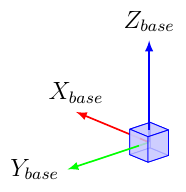
\includegraphics[width=0.15\textwidth]{chapter2/images/right_hand_rule.png}
	\caption{การตั้งแกนตามกฏมือขวา}
	\label{fig:right_hand_rule}
\end{figure}